To find the ROI that is the table there are several approaches that could be used:
\begin{itemize}
	\item Search for the table as a big rectangle.
	\item Searching for the holes on the pool table.
	\item Finding the most common colour (the cloth) and then find the outer points of the cloth.
\end{itemize}

The method of searching for the table as a big rectangle is chosen. 					%EXPLAING MORE!

The method used is explained by this flowchart\ref{fig:detecttable_flowchart}:

\begin{figure}[htpb]
\begin{center}
\leavevmode
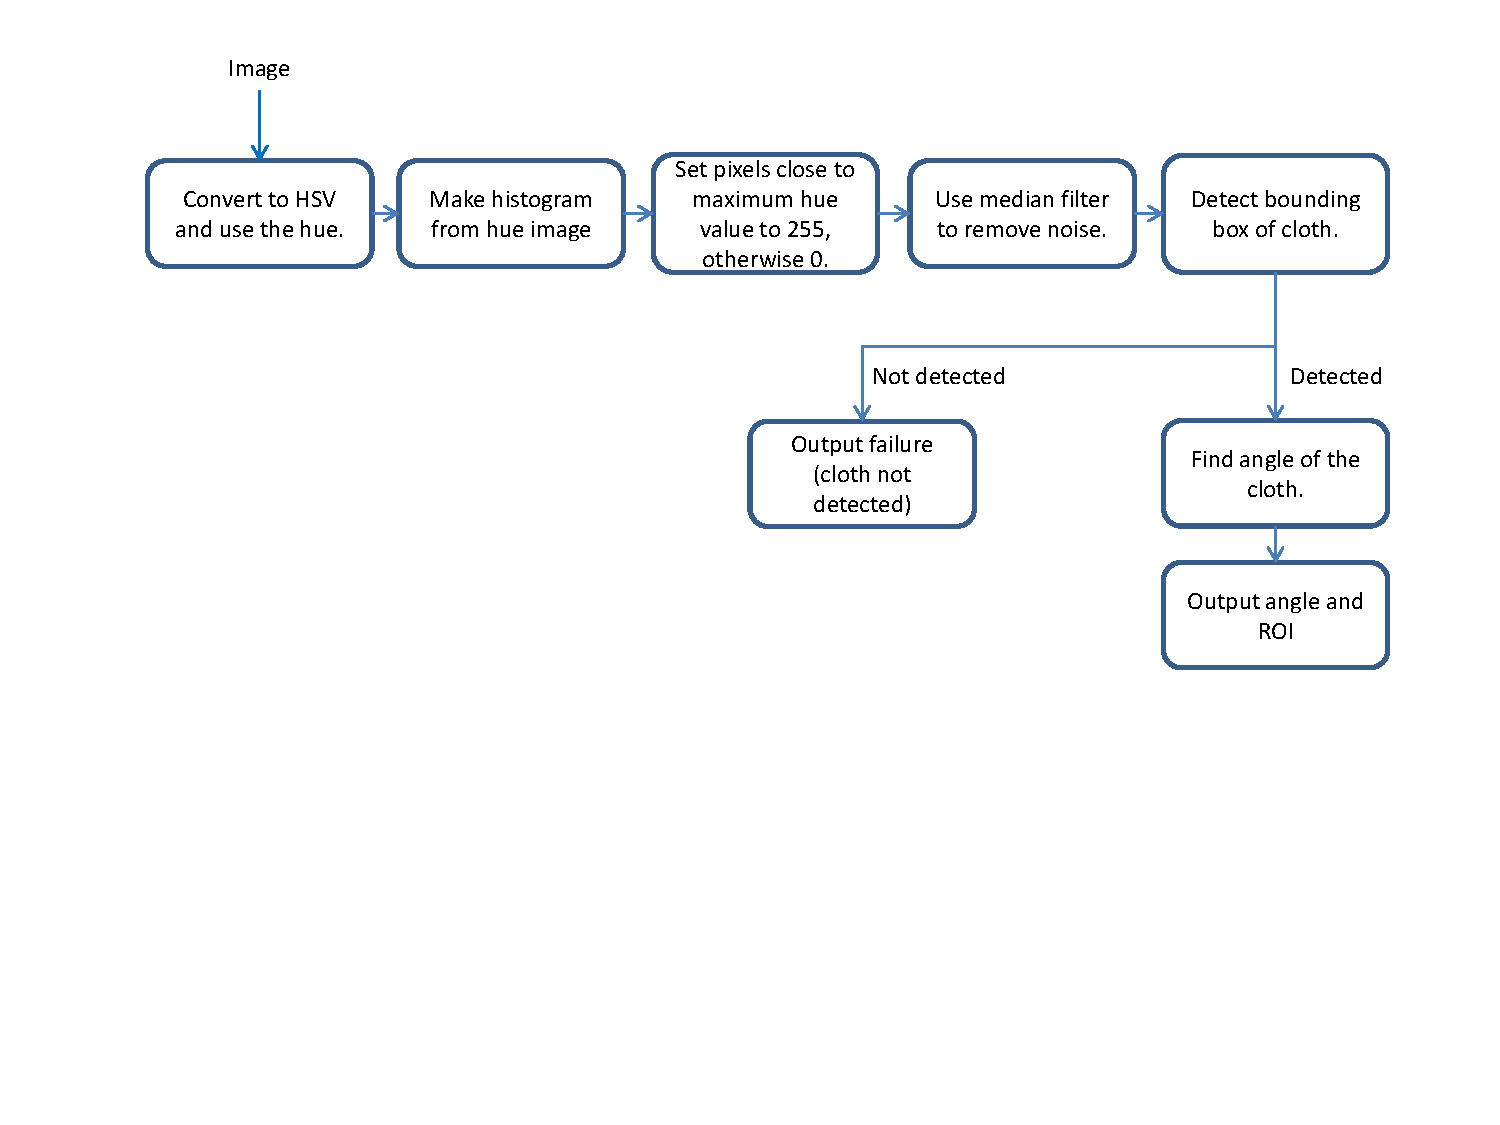
\includegraphics[width=0.5\textwidth]{images/tabledetect_flowchart.pdf}
\end{center}
\caption{Flowchart explaining table detection.}
\label{fig:detecttable_flowchart}
\end{figure}
																						%Redo IMAGE

The following steps will be done:
\begin{enumerate}

\item The input image is made binary using adaptive threshold.

\item The image is processed using a median filter and then eroded.

\item Find the contours of the image by using chain code. Secondly sort the contours by size.

\item Check if the contour is a rectangle. This is done by converting the vertices of the contour into lines. These lines should lie orthogonal to each other or a lest very close to.

\item As set in the requirements specification\ref{sec:reqspec} the table has to take up at least 75\% of the image. Therefore the limit for the size of the table after image processing is set to 50\%. If the contour found is not at least this percentage, then the ROI is returned as not found. Otherwise the ROI will be returned.
\end{enumerate}

\textbf{Adaptive threshold:}
In the requirements specification\ref{sec:reqspec} it is set that the system should work in mixed light conditions. Therefore it is crucial to have methods that work based on their surroundings. This is where adaptive threshold is a very good and simple tool.

Where normal threshold uses only one value for an entire image, adaptive threshold allows for the threshold value to change according to the surroundings. This is very good for operations that take place in scenes with different light and thereby it is more robust.

Normal thresholding is a very simple operation.

\begin{center}
	if $P(x,y) > threshold$ then $P(x,y) = 1$

	else $P(x,y) = 0$
\end{center}

Using adaptive threshold it becomes slightly more complicated. The threshold is now no longer static, but dynamic and depends on the surrounding pixels in a blocksize $b$. The blocksize $b$ is a value that determine how big a portion of the surroundings the threshold will be calculated from.

\begin{center}
	$threshold = \sum_{k=x-b}^{x+b} \sum_{j=y-b}^{y+b} P(x,y)$

	$if  P(x,y) > threshold$ then $P(x,y) = 1$

	else $P(x,y) = 0$
\end{center}

Furthermore it is possible to select if the mean should be a equally weighted mean or if it should be a Gaussian mean which would put the closest pixels to more importance.

An example of using adaptive threshold can be seen here and it is easy to see the big advantage of adaptive threshold\ref{fig:adaptivethreshold}. 

\begin{figure}[htpb]
\begin{center}
\leavevmode
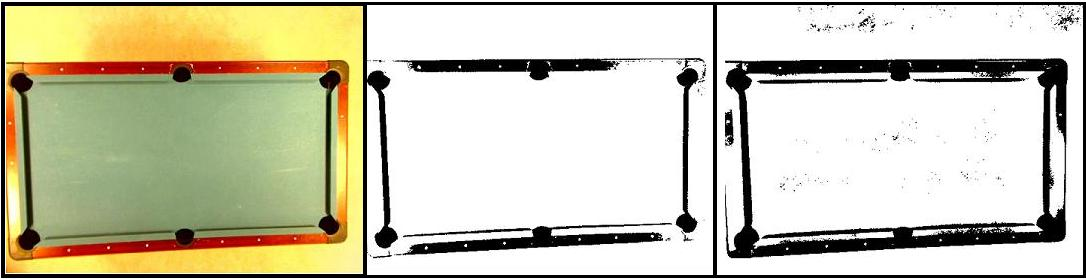
\includegraphics[width=1\textwidth]{images/adaptive_threshold.JPG}
\end{center}
\caption{First image not processed, second is normal threshold and third is using adaptive threshold}
\label{fig:adaptivethreshold}
\end{figure}

In this example the objective was to find the table and this is better accomplished using adaptive threshold. If the light would have been the same in every part of the input image then normal threshold would have been just as good, but the light often would not be. The noise introduced by adaptive thresholding, as seen in the top right corner, can easily be removed with a standard median filter.

\textbf{Median filter and SOMETING:}
To remove noise a median filter is applied to the image. This will remove noise and have no impact other places.
Then to make the contour bigger the image is ERODED/DILATED.

INSERT IMAGE

\textbf{Finding contours:}
Finding contours is 
